\documentclass[a4paper,12pt]{article}

\RequirePackage{epsfig}
\usepackage{graphicx}

\setlength\hoffset{-0.5in}      %% these work quite well with a 12pt font
\setlength\voffset{-0.5in}
\setlength{\textwidth}{6.30in}
\setlength{\textheight}{9.0in}

\bibliographystyle{unsrt}

\begin{document}

\begin{center}
{\Large\bf{Planning the Seating Chart for Optimal Weddings}} \\
      \vspace{5.0mm}
{\Large\bf{Project Plan}} \\
      \vspace{8mm}
      {\large\bf{Daniel Joffe}}  \\
      \vspace{5.0mm}
       {\tt u03dj17@abdn.ac.uk} \\
      \vspace{5.0mm}
      {\em Department of Computing Science,\\
       University of Aberdeen, Aberdeen AB24 3UE, UK} 
\end{center}


\section*{Introduction}
A staple part of weddings is the dinner, during which guests
are grouped together and sat at tables for the duration of
the meal. Most people would prefer to eat with close friends
and family rather than with strangers or bitter enemies. In
the latter case, it may not be only those sat together who have
a bad time, but everyone within earshot as well.

In weddings with upwards of a hundred guests, finding an
arrangement that makes everyone happy can be a difficult task.
Care must be taken to ensure that everyone is sat with as many
friends as possible and away from any nemeses they might have.
Matters are complicated further when two people who hate each
other have a mutual friend. Many hours have been spent wrangling
complex relationship networks into an amenable seating chart and
the failure to do so has ruined many weddings.

The purpose of this project is to automate the process, so that
good seating charts can be found faster than humanly possible and
so that wedding planners can be assured knowing that their seating
plan is (among) the best possible for their particular problem
instance.

Though framed in the language of weddings, the underlying problem
is relevant to other areas. In universities, professors may wish
to find a composition of teams for a group project that results in
minimal in-fighting. A safari park may want to find some way of
grouping different animals together such that minimal land needs
to be bought, while maintaining that none of them eat each other.

\section*{Goals}

The ultimate goal is to find an efficient heuristic for solving the seating
chart problem and to assess its feasibility in terms of correctness and
computational resources. To this end, I intend to verify the results of Meghan
L. Bellows and J. D. Luc Peterson (cite this) and compare their approach to
standard metaheuristics such as genetic algorithms and hill climbing.

\subsection*{Strech Goals}

The following goals would be nice to achieve if possible, but are low-priority:

\begin{itemize}
\item Produce a usable tool with an interface for non-experts to generate
      seating charts for their real weddings.
\item Consider more refined models of the problem, such as accounting for
      variably-sized dinner tables.
\end{itemize}

\section*{Methodology}

The steps that I plan to take to achieve my goals are as follows. If a problem
is found in a previous step, it will be remedied, and any steps relying on it
will be revised.

\begin{itemize}
\item Read previous works relating to combinatorial optimisation problems.
\item Formalise the metrics that will be used to evaluate different heuristics for
      this problem.
\item Select and implement at least 3 different heuristics. This will require
      learning the use of various software libraries.
\item Test heuristics on hand-crafted problem instances to verify their soundness.
\item Generate a large number of larger problem instances.
\item Test the implemented heuristics on the larger dataset.
\item Compare the implemented heuristics by the metrics previously decided on.
\item Write a report detailing the process, conclusions, and suggesting areas of
      further research.
\end{itemize}

\section*{Resources Required}

I will require a development computer with a general-purpose programming
language installed, such as Python or Rust. I will need access to integer
programming software such as IBM's CPLEX or Google's OR-tools. For some
testing, I may need access to a high performance computing service such
as the University of Aberdeen's Maxwell.

\section*{Risk Assessment}

Try to describe possible circumstances (e.g. a particular piece of
technology doesn't work or is too expensive) that might cause
the project to become become infeasible. What would you have to do
or change to recover your project?

\section*{Timetable}

This section should describe the {\em schedule} for your project. 
You should describe the various activities you expect to perform
and their durations, along with any deadlines and deliverables.
It is often useful to collect all of this information in a
{\em Gantt chart}, as shown in Figure~\ref{fig:plan} below:

\begin{figure}[htb]
\begin{center}
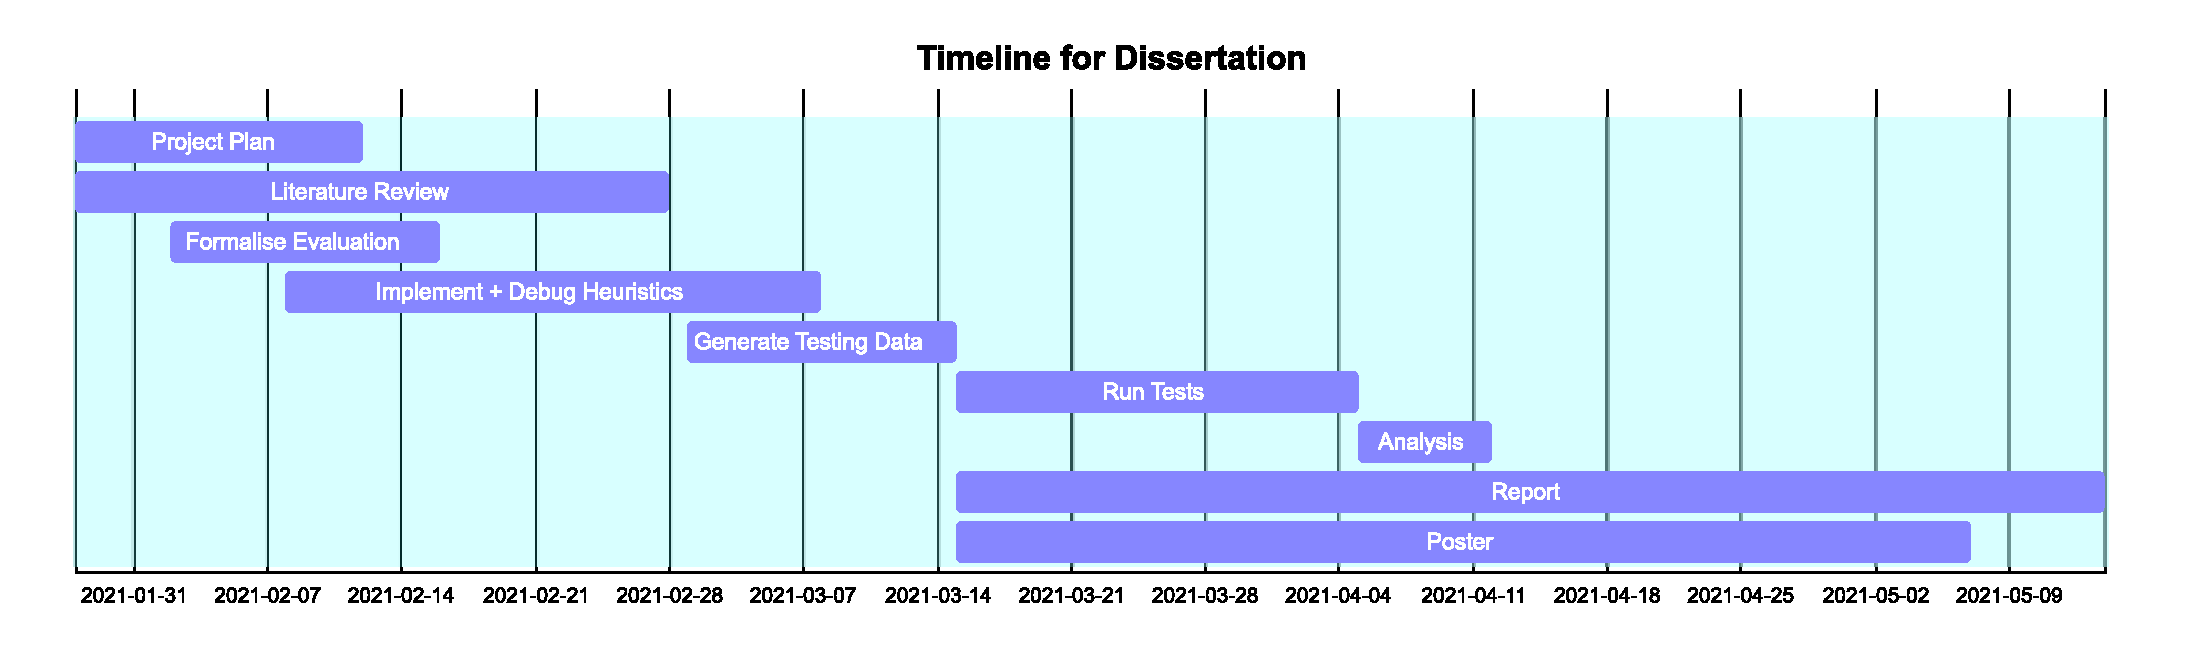
\includegraphics[scale=0.4]{gantt.eps}
\caption{Main Project Activities\label{fig:plan}}
\end{center}
\end{figure}

% For information, this figure was created using xfig, and 
% converted to encapsulated postscript by a command in the Makefile
% before being included as a graphic in the \LaTeX document.

Don't forget to add time at the end of your project for 
evaluation and writing-up! This could easily require 2-3 weeks.


\bibliography{ProjectPlan}

\end{document}
